\chapter{H\"older Continuity for HR}

\section{Introduction}
%
%
%
We consider the hyperelastic rod (HR) Cauchy problem
\begin{gather}
 \p_t u =  -\gamma u \p_x u -
 \p_{x} D^{-2} \left[ \frac{3-\gamma}{2}u^2 +
\frac{\gamma}{2} \left( \p_x u \right)^2
\right],
\label{hyperelastic-rod-equation-b}
\\
 u(x,0) = u_0(x), \; \; x \in \rr, \; \; t \in \rr
\label{init-cond-b}
\end{gather}
%
%
where 
\begin{equation*}
	D^{m} = (1 - \p_x^2)^{m/2}, \quad m \in \rr
\end{equation*}
and  $\gamma$  is a  nonzero constant. The HR equation was first
derived by Dai in \cite{Dai_1998_Model-equations} as a one-dimensional 
model for finite-length and
small-amplitude axial deformation waves in thin cylindrical
rods composed of a compressible Mooney-Rivlin
material. The derivation relied upon a reductive perturbation technique, 
and took into account the nonlinear dispersion of pulses propagating 
along a rod. It was assumed that each cross-section of the rod is 
subject to a stretching and rotation in space. The solution $u(x,t)$ to the 
HR equation represents the radial stretch relative
to a pre-stressed state, while $\gamma$ is a fixed constant depending upon 
the pre-stress and the material used in
the rod, with values ranging from $- 29.4760$ to $3.4174$.
%
\\
\\
The well-posedness of the HR equation has been studied by several authors. 
In Yin \cite{Yin_2003_On-the-Cauchy-p} and Zhou 
\cite{Zhou_2005_Local-well-pose}, a proof of local well-posedness in Sobolev 
spaces $H^s$,  $s > 3/2$, is described  on the line and the circle, respectively. 
Their approach is to rewrite the HR equation   
in its non-local form, and then to verify the conditions needed to apply 
Kato's semi-group theory \cite{Kato_1975_Quasi-linear-eq}. Using an alternative,
Galerkin type method outlined in Taylor \cite{Taylor_1991_Pseudodifferent}, local
well-posedness in Sobolev spaces $H^s$,  $s > 3/2$ on the line and the circle is
established in \cite{Karapetyan:2010fk}. 
For details on how this is done for CH ($\gamma =1$) on the line, see Rodriguez-Blanco 
\cite{Rodriguez-Blanco_2001_On-the-Cauchy-p}. Blow-up criteria 
is also investigated in \cite{Yin_2003_On-the-Cauchy-p} and 
\cite{Zhou_2005_Local-well-pose}, as well as by Constantin and Strauss 
\cite{Constantin_2000_Stability-of-a-}. 
\\
\\
Setting $\gamma = 0$ gives the celebrated 
BBM equation, which was proposed by 
Benjamin, Bona, and Mahony 
\cite{Benjamin_1972_Model-equations} as a model for 
the unidirectional evolution of long waves.
Solitary-wave solutions to this 
equation are global and orbitally stable (see Benjamin 
\cite{Benjamin_1972_The-stability-o}, 
\cite{Benjamin_1972_Model-equations}, and 
\cite{Constantin_2000_Stability-of-a-}).
For more general $\gamma$, the existence of global 
solutions to HR on the line with constant $H^1$ energy
was proved recently by Mustafa \cite{Mustafa_2007_Global-conserva}
using the approach developed by Bressan and 
Constantin in \cite{Bressan_2007_Global-conserva}. Using a vanishing 
viscosity argument, Coclite, 
Holden, and Karlsen \cite{Coclite_2005_Global-weak-sol}
established existence of a strongly continuous semigroup of global 
weak solutions of HR on the line for initial data in $H^1$.
Bendahmane, Coclite, and Karlsen 
\cite{Bendahmane_2006_Hsp-1-perturbat} extended this result to traveling 
wave solutions that are supersonic solitary shockwaves.
For more information on the existence of global solutions to the HR
equation, see Holden and Raynaud \cite{Holden_2007_Global-conserva}
and \cite{Yin_2003_On-the-Cauchy-p}. 
\\
\\
There is a variety of traveling wave solutions to the HR equation that can be 
obtained using various combinations of peaks, cusps, compactons, 
fractal-like waves, and plateaus (see Lenells 
\cite{Lenells_2006_Traveling-waves}). Orbital stability of solitary wave 
solutions was proved in \cite{Constantin_2000_Stability-of-a-}.
Solitary shock wave formation was 
analyzed in Dai and Huo \cite{Dai_2000_Solitary-shock-} using traveling 
wave solutions of the HR equation to derive a system of ordinary differential 
equations, with a vertical singular line in the phase plane corresponding with the 
formation of shock waves. Head-on collisions between two solitary 
waves was investigated in the work of Hui-Hui Dai, 
Shiqiang Dai, and Huo \cite{Dai_2000_Head-on-collisi} using a reductive 
perturbation method coupled with the technique of strained coordinates. 
\\
\\
In this work we study the continuity properties of the data-to-solution map for the HR 
equation, expanding upon the work in \cite{Karapetyan:2010fk}, in which it was
shown that the data-to-solution map is not better than continuous in Sobolev
spaces $H^{s}$ on the line
and the circle. More precisely, following \cite{Chen:2011fk} we show the following result:
%
%
\begin{theorem}[H\"older Continuity]
  For $\gamma \neq 0$, the
  data to solution map for HR is H\"older continuous from $B_{H^{s}}(R)$ (in
  the topology of $H^{r}$) to $C([0, T], H^{r})$, where $T = T(R)$, for $s >
  3/2$, $-1 \le r < s$. More
  precisely, decompose the set $\Omega = \left\{ (s, r) \in \rr^{2}  \right\}$
  into the pieces
  %
  %
  \begin{equation*}
  \begin{split}
    & \Omega_{1} = \left\{ (s, \ r):  \ s < 3/2 \right\}
    \\
    & \Omega_{2} = \left\{ (s, \ r):
     \ s>3/2, \ r < -1  \right\}
    \\
    & \Omega_{3} = \left\{ (s, \ r):
     \ s>3/2, \ r > s  \right\}
    \\
    & \Omega_{4} = \left\{ (s, \ r):
     \ s>3/2, \ -1 \le r \le s-1, \ s + r \ge 2  \right\}
    \\
    & \Omega_{5} = \left\{ (s, \ r):
     \ s>3/2, \ -1 \le r < 2-s \right\}
    \\
    & \Omega_{6} = \left\{ (s, \ r):
    \  s>3/2, \  s-1 < r < s  \right\}.
    \end{split}
\end{equation*}
  %
  %
\label{thm:main-thm}
\end{theorem}
%
\begin{center}
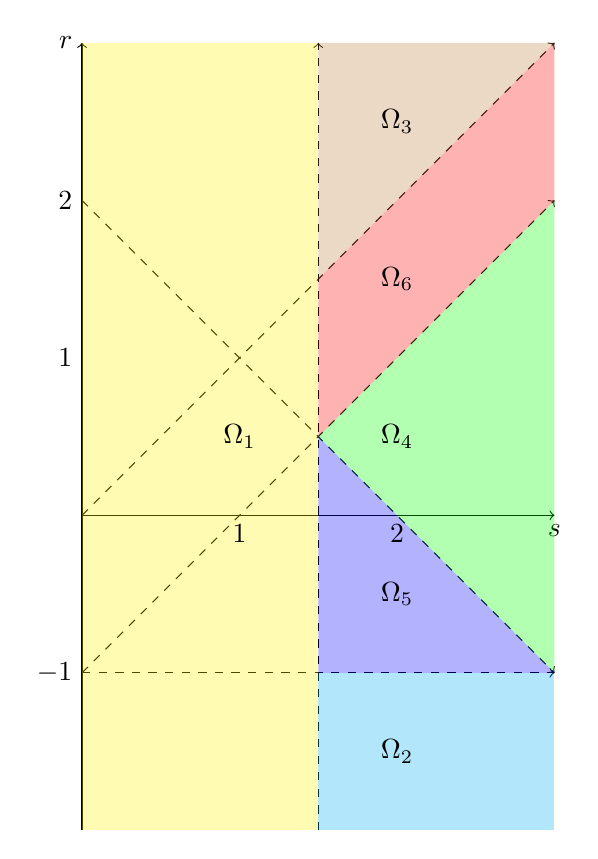
\begin{tikzpicture}[scale=2]
% Draw thin grid lines with color 40% gray + 60% white

% Draw x and y axis lines
\draw [->] (0,0) -- (3,0) node [below] {$s$};
\draw [->] (0,-2) -- (0,3) node [left] {$r$};
\draw [->, dashed] (0,0) -- (3,3) ;
\draw [->, dashed] (0,-1) -- (3,2) ;
\draw [->, dashed] (0,2) -- (3,-1) ;
\draw [->, dashed] (0,-1) -- (3,-1) ;
\draw [->, dashed] (3/2,-2) -- (3/2, 3);
\fill[color=green, fill opacity=0.3] (1.5, 0.5) -- (3,2) -- (3,0) -- (3,-1);
\fill[color=red, fill opacity=0.3] (1.5, 0.5) -- (1.5,1.5) -- (3,3) -- (3,2);
\fill[color=yellow, fill opacity=0.3] (0, -2) -- (1.5, -2) -- (1.5, 3) -- (0, 3);
\fill[color=blue, fill opacity=0.3] (1.5, 0.5) -- (1.5, -1) -- (3, -1);
\fill[color=brown, fill opacity=0.3] (1.5, 1.5) -- (3, 3) -- (1.5, 3);
\fill[color=cyan, fill opacity=0.3] (1.5, -1) -- (3, -1) -- (3, -2) -- (1.5, -2);


\foreach \x/\xtext in { 1, 2}
    \draw[shift={(\x,0)}]  node[below] {$\xtext$};
\foreach \y/\ytext in {-1, 1, 2}
    \draw[shift={(0,\y)}]  node[left] {$\ytext$};
    \draw (1,0.5) node {$\Omega_{1}$};
    \draw (2,2.5) node {$\Omega_{3}$};
    \draw (2,1.5) node {$\Omega_{6}$};
    \draw (2,-1.5) node {$\Omega_{2}$};
    \draw (2,0.5) node {$\Omega_{4}$};
    \draw (2,-0.5) node {$\Omega_{5}$};
\end{tikzpicture}
\end{center}
%
%
Then for two initial data $u_{0}, v_{0} \in B_{H^{s}}(R)$, there exist unique
corresponding solutions $u(x,t), v(x,t)$ for $0 \le t \le T= T(R)$ to the
HR equation \eqref{hyperelastic-rod-equation-b} which satisfy 
%
%
\begin{equation*}
\begin{split}
  \| u(t) - v(t) \|_{H^{r}} \le C \| u_{0} - v_{0} \|^{\alpha(s, r, \gamma)},
  \quad 0
  \le t \le T
\end{split}
\end{equation*}
%
%
where 
%
%
\begin{equation*}
\begin{split}
\alpha = 
\begin{cases}
   1, \quad & (s,r, \gamma) \in \Omega_{4} 
  \\
   2(s-1)/(2-r),  \quad & (s, r, \gamma) \in \Omega_{5}
  \\
   s-r, \quad & (s, r, \gamma) \in \Omega_{6}.
\end{cases}
\end{split}
\end{equation*}

%
%%%%%%%%%%%%%%%%%%%%%%%%%%%%%%%%%%%%%%%%%%%%%%%%%%%%%
%
%
%                Main theorem
%
%
%%%%%%%%%%%%%%%%%%%%%%%%%%%%%%%%%%%%%%%%%%%%%%%%%%%%%
%
%
We remark that this result improves upon the H\"older continuity result in
\cite{Chen:2011fk} (there it is for $0 \le r < s$) by a full degree in $r$. 
%
%
%
%
\section{Proof of \hyperref[thm:main-thm]{H\"older Continuity}}
%
%
The proof in the periodic case is analogous to that in the non-periodic case.
Hence, we restrict our attention to the non-periodic case. 

%
%
\subsection{Region $\Omega_{1}$} 
\label{ssec:reg-2}
This is open. In particular, well-posedness of HR must be proved or disproved
below $3/2$ before we can even consider discussing H\"older continuity in weak
topologies.
\subsection{Region $\Omega_{2}$} 
\label{ssec:reg-6}
Open. The lower bound on $r$ comes from Lemma \ref{cor1-b}. Perhaps the lemma can
be strengthened.
\subsection{Region $\Omega_{3}$} 
\label{ssec:reg-7}
It makes little sense to talk about this region, 
i.e. we assume a priori that our initial
data is in $H^{s}$ (i.e. it may not even be in $H^{r}$ if $r > s$). If it is in
$H^{r}$, then we are back where we started.
\subsection{Region $\Omega_{4}$} 
\label{ssec:reg-m-imp}
%
%
Let $u_{0}(x), v_{0}(x)
\in B_{H^{s}}(R)$, $s > 3/2$ be two initial datum. Then from
the well-posedness theory for HR \cite{Karapetyan:2010fk}, we
know that there exists unique corresponding solutions $u, v \in C(I,
B_{H^{s}}(2R))$ to \eqref{hyperelastic-rod-equation-b}.
Set $v=u-w$. Then $v$ solves the Cauchy-problem
%
%
\begin{align}
	\label{uniqueness-exp-b}
& \p_t v
=  -\frac{\gamma}{2} \p_x [v(u + w)] 
\\
\notag
& \phantom{\p_t v = }- D^{-2} \p_x \left\{
\frac{3-\gamma}{2}[v(u+w)] + \frac{\gamma}{2}[\p_x v \cdot \p_x (u+w)]
\right\},
\\
& v(x,0) = u_{0}(x) - v_{0}(x).
\label{uniqueness-init-data-b}
\end{align}
%
%
%
%
Applying $D^r$ to both sides of \eqref{uniqueness-exp-b}, then 
multiplying both sides by $D^r v$ and integrating, we obtain
%
%
\begin{equation}
\begin{split}
 \frac{1}{2} \frac{d}{dt} \|v\|_{H^r}^2
 = & -\frac{\gamma}{2} \int_{\rr} D^r \p_x [v(u+w)] \cdot
D^r v \ dx
\\
& - \frac{3-\gamma}{2} \int_{\rr}  D^{r -2}
\p_x[v(u+w)] \cdot
D^r v \ dx  
\\
& - \frac{\gamma}{2} \int_{\rr} D^{r 
-2} \p_x [ \p_x v
\cdot \p_x (u+w)]\cdot D^r v \ dx .
\label{2v-b}
\end{split}
\end{equation}
%
%
We now estimate \eqref{2v-b} in parts.

\subsection{Estimate of Integral 1} Note that
%
%
\begin{equation}
\begin{split}
& \left |  -\frac{\gamma}{2} \int_{\rr} D^r \p_x [v(u+w)] \cdot
D^r v \ dx \right |
\\
& =
\left |
-\frac{\gamma}{2} \int_{\rr} \left[ D^r \p_x, \ u+w \right]v \cdot
D^r v \ dx - \frac{\gamma}{2} \int_{\rr} (u+w) D^r
\p_x v \cdot D^r v\ dx
\right | \\
& \le \left |
-\frac{\gamma}{2} \int_{\rr} \left[ D^r \p_x, \ u+w \right]v \cdot
D^r v \ dx \right |
+ \left | \frac{\gamma}{2} \int_{\rr} (u+w) D^r \p_x v
\cdot D^r v\
dx \right |.
\label{4v-b}
\end{split}
\end{equation}
%
%
Observe that integrating by parts gives
%
%
\begin{equation}
\begin{split}
\left | \frac{\gamma}{2}\int_{\rr} (u+w) D^r \p_x v \cdot
D^r v \ dx \right |
\lesssim \|\p_x (u+w)\|_{L^\infty}
\|v\|_{H^r}^2.
\label{4'v-b}
\end{split}
\end{equation}
%
%
%
%
To estimate the remaining integral of \eqref{4v-b}, we shall need the following
following result taken from \cite{Himonas_2009_Non-uniform-dep-per}:
%
\begin{lemma}
\label{cor1-b}
If $s > 3/2$ and $-1 \le r  \le s -1$, then
%
%
\begin{equation}
\begin{split}
\|[D^r \p_x ,f]g\|_{L^2} \le C \|f\|_{H^s} \|g\|_{H^r}.
\label{15-b}
\end{split}
\end{equation}
%
%
\end{lemma}
%
%
Set $s > 3/2$ and $-1 \le r \le s -1$. An application of 
Cauchy-Schwartz and Lemma \ref{cor1-b} then yields 
%
%
\begin{equation}
\begin{split}
 \left | -\frac{\gamma}{2} \int_{\rr} [D^r \p_x, \ u+w] v
\cdot D^r v \ dx \right |
& \lesssim \|u+w\|_{H^s} 
\|v\|_{H^r}^2.
\label{7v-b}
\end{split}
\end{equation}
%
%
Combining \eqref{4'v-b} and \eqref{7v-b} and applying the Sobolev Imbedding 
Theorem, we obtain the estimate
%
%
\begin{equation}
\begin{split}
\left |  -\frac{\gamma}{2} \int_{\rr} D^r \p_x [v(u+w)] \cdot
D^r v \ dx \right |
 \lesssim \|u+w\|_{H^s} \|v\|_{H^r}^2, \quad s > 3/2, \ -1 \le r \le s-1.
\label{8v-b}
\end{split}
\end{equation}
%
%

\subsection{Estimate of Integral 2} We shall need the following.
%
%
%%%%%%%%%%%%%%%%%%%%%%%%%%%%%%%%%%%%%%%%%%%%%%%%%%%%%
%
%
%                frac deriv est
%
%
%%%%%%%%%%%%%%%%%%%%%%%%%%%%%%%%%%%%%%%%%%%%%%%%%%%%%
%
%
\begin{lemma}
For $s > 3/2$, $r \le s$, $s + r \ge 2$, we have
%
%
\begin{equation*}
\begin{split}
  \| fg \|_{H^{r-1}} \le \| f \|_{H^{r-1}} \| g \|_{H^{s}}.
\end{split}
\end{equation*}
%
%
\label{lem:frac-deriv}
\end{lemma}
%
%
%
%
%
%
Applying Cauchy-Schwartz and Lemma \ref{lem:frac-deriv}, we obtain
%
%
%
\begin{equation*}
\begin{split}
\left | - \frac{3-\gamma}{2} \int_{\rr}  D^{r -2}
\p_x[v(u+w)] \cdot
D^r v \ dx  \right |
 & \lesssim \|u+w\|_{H^{r -1}} \|v\|_{H^r}^2
\end{split}
\end{equation*}
%
%
which implies
\begin{equation}
\begin{split}
\left | - \frac{3-\gamma}{2} \int_{\rr}  D^{r -2}
\p_x[v(u+w)] \cdot
D^r v \ dx  \right |
 & \lesssim \|u+w\|_{H^{s}} \|v\|_{H^r}^2
 \label{3v-b}
\end{split}
\end{equation}
%
for $s > 3/2, \ r \le s, \ \text{and} \ s + r \ge 2$.
%
%
\subsection{Estimate of Integral 3} We first apply
Cauchy-Schwartz to obtain
%
%
\begin{equation*}
\begin{split}
\left | - \frac{\gamma}{2} \int_{\rr} D^{r 
-2} \p_x [ \p_x v
\cdot \p_x (u+w)]\cdot D^r v \ dx \right | 
 \lesssim 
\|[\p_x v \cdot \p_x (u+w)] \|_{H^{r -1}}
\|v\|_{H^r}.
\end{split}
\end{equation*}
%
We now need the following result.
%
%
%
\begin{lemma}
\label{impo-b}
If  $s > 3/2$, $r \le s$, and $s + r \ge 2$,  then
%
%
\begin{equation}
\begin{split}
  \|f_{x}g_{x}\|_{H^{r - 1}} \le C \|f\|_{H^{r}}
\|g\|_{H^{s}}.
\label{11-bb}
\end{split}
\end{equation}
%
%
\end{lemma}
%
Applying the lemma, we conclude that
%
\begin{equation}
\begin{split}
\left | - \frac{3-\gamma}{2} \int_{\rr}  D^{r -2}
\p_x[v(u+w)] \cdot
D^r v \ dx  \right |
 \lesssim \|u+w \|_{H^{s}}
\|v\|_{H^r}^2
\label{3'v-b}
\end{split}
\end{equation}
%
%
for $s > 3/2, \ r \le s, \ \text{and} \ s + r \ge 2$.
%
%
%
%
Grouping \eqref{8v-b}, \eqref{3v-b}, and \eqref{3'v-b}, and 
applying
the Sobolev Imbedding Theorem, we obtain
%
%
\begin{equation}
\begin{split}
\frac{1}{2} \frac{d}{dt}
\|v\|_{H^r}^2
& \lesssim \|u+w\|_{H^s}
\|v\|_{H^r}^2, \quad | t | < T
\\
& \le 2R \| v \|_{H^{r}}^{2}.
\label{9vbb}
\end{split}
\end{equation}
%
%
%
%
%
Letting $y(t) = \| v \|^{2}_{H^{r}}$, we obtain
%
%
%
\begin{equation*}
\begin{split}
  \frac{dy}{dt} \le cy
\end{split}
\end{equation*}
%
where $c = c(s, r, R)$. 
This admits the solution
%
%
\begin{equation*}
\begin{split}
  y(t) \le y(0) e^{ct}, \quad | t | < T
\end{split}
\end{equation*}
%
%
which implies
%
%
\begin{equation*}
\begin{split}
  y(t) \le y(0) e^{cT}.
\end{split}
\end{equation*}
%
%
Substituting back in for $y$, we see that
%
%
\begin{equation*}
\begin{split}
  \| v \|_{H^{r}}^{2} \le \| v(0) \|^{2}_{H^{r}} e^{cT}
\end{split}
\end{equation*}
%
%
or
%
%
\begin{equation}
  \label{lip-ineq}
\begin{split}
  & \| u(t) - w(t) \|_{H^{r}} \le C \| u_{0} - w_{0} \|_{H^{r}}, 
  \\
  & \text{for} \ | t | < T,
  \ s > 3/2, \ -1 \le r \le s-1, \ s + r \ge 2.
\end{split}
\end{equation}
%
Hence, in region $\Omega_{4}$, the data to solution map is locally Lipschitz from
$B_{H^{s}(R)}$ (in the $H^{r}$
topology) to $C([-T, T], H^{r})$, with Lipschitz constant $C = C(s, r, R)$.
%
%
%
%
%
%
%
%
%
%
\subsection{Region $\Omega_{5}$} 
\label{ssec:case-4}
%
%
Note that   $-1 \le 2-s \le s-1$ for $s>3/2$ and $s + (2-s) = 2$.
Hence, applying \eqref{lip-ineq}, we bound 
%
%
%
%
\begin{equation}
  \label{fgh}
\begin{split}
  \| v(t) \|_{H^{r}}
  & \le \|v(t) \|_{H^{2-s}}
  \\
  & \lesssim \|v(0) \|_{H^{2-s}}.
  \end{split}
\end{equation}
%
We need the following interpolation
result. 
%
%
%%%%%%%%%%%%%%%%%%%%%%%%%%%%%%%%%%%%%%%%%%%%%%%%%%%%%
%
%
%                interp
%
%
%%%%%%%%%%%%%%%%%%%%%%%%%%%%%%%%%%%%%%%%%%%%%%%%%%%%%
%
%
\begin{lemma}
  For $m_{1} < m < m_{2}$,
  %
  %
  \begin{equation*}
  \begin{split}
    \| f \|_{H^{m}} \le \| f \|_{H^{m_{1}}}^{(m_{2}-m)/(m_{2} - m_{1})} \| f
    \|_{H^{m_{2}}}^{(m -m_{1})/(m_{2} - m_{1})}.
  \end{split}
  \end{equation*}
  %
  %
  %
  %
   %
  %
\label{lem:interp}
\end{lemma}
%
Applying the lemma with $m_{1} =r$, $m = 2-s$, and $m_{2} = s$, we bound \eqref{fgh} by
%
%
\begin{equation*}
\begin{split}
  \| v(0) \|_{H^{r}}^{\frac{2(s-1)}{2-r}} \|v(0)
  \|_{H^{s}}^{\frac{2-s-r}{s-r}}
  & = \| u_{0} - w_{0} \|_{H^{r}}^{\frac{2(s-1)}{2-r}} \|u_{0} - w_{0}
  \|_{H^{s}}^{\frac{2-s-r}{s-r}}
  \\
  & \lesssim \| u_{0} - w_{0} \|_{H^{r}}^{\frac{2(s-1)}{2-r}}.
\end{split}
\end{equation*}
%
We conclude that
%
%
\begin{equation*}
\begin{split}
  \| u(t) - w(t) \|_{H^{r}} \lesssim \|u_{0} - w_{0} \|_{H^{r}}^{\frac{2(s-1)}{2-r}}.
\end{split}
\end{equation*}
%
%
%
%
\subsection{Region $\Omega_{6}$} 
\label{ssec:case-2}
%
%
Applying Lemma \ref{lem:interp} and the fact that 
%
%
\begin{equation*}
\begin{split}
  \|v\|_{H^{s}} = \|u - w \|_{H^{s}} \le 4R
\end{split}
\end{equation*}
%
%
we obtain
%
%
\begin{equation}
  \label{pre-lip-ap}
\begin{split}
  \| v(t) \|_{r} & \lesssim \| v(t) \|_{H^{s-1}}^{s-r} \|v(t) \|_{H^{s}}^{1-s+r}
  \\
  & \simeq \| v(t) \|_{H^{s-1}}^{s-r}.
\end{split}
\end{equation}
%
%
Notice that $-1 \le s-1 \le s-1$, and $s + (s-1) = 2s-1 \ge 2$ for $s >3/2$.
Hence, we may apply \eqref{lip-ineq} to bound \eqref{pre-lip-ap} by
%
%
\begin{equation*}
\begin{split}
  C \|v(0) \|_{H^{s-1}}^{s-r}
  & \lesssim \|v(0) \|_{H^{r}}^{s-r} 
  = \|u_{0} - w_{0}\|_{H^{r}}^{s-r}.
\end{split}
\end{equation*}
%
%
This completes the proof of Theorem \ref{thm:main-thm}. \qed
%
%%%%%%%%%%%%%%%%%%%%%%%%%%%%%%%%%%%%%%%%%%%%%%%%%%%%%
%
%
%                proofs of lemmas
%
%
%%%%%%%%%%%%%%%%%%%%%%%%%%%%%%%%%%%%%%%%%%%%%%%%%%%%%
%
%
\section{Proofs of Lemmas} 
\label{sec:pf-lemmas}
%
%
%
\begin{proof}[Proof of Lemma \ref{lem:frac-deriv}]
For the non-periodic case we have
%
%
\begin{equation*}
\begin{split}
  \| fg\|_{H^{r-1}}^{2}
  & = \int_{\rr} (1 + \xi^{2})^{r-1}| \int_{\rr}
  \wh{f}(\eta) \wh{g}( \xi - \eta) d \eta |^{2} d \xi
  \\
  & \le \int_{\rr} (1 + \xi^{2})^{r-1}\left [ \int_{\rr}
  | \wh{f}(\eta) |  | \wh{g}(\xi - \eta) | 
  d \eta \right ]^{2} d \xi
  \\
  & = \int_{\rr}  (1 + \xi^{2})^{r-1}\left [ \int_{\rr}
  | \wh{f}(\eta) |  | \wh{g}(\xi - \eta) | (1 +
  \eta^{2})^{\frac{1-s}{2}} (1 + \eta^{2})^{\frac{s-1}{2}}
  d \eta \right ]^{2} d \xi
  \\
  & \le \int_{\rr}  (1 + \xi^{2})^{r-1}\left [ \int_{\rr} 
  | \wh{f}(\eta) | | \wh{g}(\xi - \eta) | (1 +
  \eta^{2})^{\frac{1-s}{2}} (1 + \eta^{2})^{\frac{s}{2}}
  d \eta \right ]^{2} d \xi.
\end{split}
\end{equation*}
%
Applying Cauchy Schwartz in $\eta$, we bound this by
%
%
%
\begin{equation}
  \label{np-key-term}
\begin{split}
  \| f \|_{H^{s}}^{2} \int_{\rr}  (1 + \xi^{2})^{r-1}\int_{\rr} \frac{|
  \wh{g}(\xi - \eta) |^{2}}{(1 + \eta^{2})^{s-1}} d \eta d \xi.
  \end{split}
\end{equation}
%
%
Applying a change of variable, we get
%
\begin{equation*}
\begin{split}
  \| f \|_{H^{s}}^{2} \int_{\rr} (1 + \xi^{2})^{r-1} \int_{\rr} \frac{
  | \wh{g}(\eta) |^{2}}{[1 + (\xi - \eta)^{2}]^{s-1}} d \eta d \xi
  \end{split}
\end{equation*}
which by Fubini is equal to
%
%
\begin{equation}
  \label{int-pre-calc-lem}
\begin{split}
  \|f \|_{H^{s}}^{2} \int_{\rr} | \wh{g}(\eta) |^{2} \int_{\rr} \frac{1}{\left[
  1 + (\xi - \eta)^{2} \right]^{s-1} (1 + \xi^{2})^{1-r}} d \xi d \eta.
\end{split}
\end{equation}
%
%
We now need the following lemma, whose proof is provided in the appendix.
%
%
\begin{lemma}
	\label{lem:calc}
 %
 Fix $p, q > 0$ such that $p +q >1$, and let $r =\min\left\{p, q, p+q-1
 \right\}$. Adopt the notation
 $\langle x - \alpha \rangle  \doteq 1 + | x - \alpha |$. Then 
 %
 \begin{enumerate}[(I)]
   \item
For $\alpha=\beta \ \text{or} \ p \neq 1 \ \text{or} \ q \neq 1$
 \begin{equation*}
\begin{split}
  & \int_{\rr} \frac{1}{\langle x - \alpha \rangle ^{p} \langle x -
  \beta \rangle
  ^{q}} d x
  \le \frac{c_{p,q}}{\langle \alpha - \beta \rangle ^{r}}, 
  \end{split}
\end{equation*}
  \item
    \begin{equation*}
  \int_{\rr} \frac{1}{\langle x - \alpha \rangle  \langle x - \beta
  \rangle} d x
  \le  \frac{4 \log \langle \alpha - \beta \rangle}{\langle \alpha - \beta
  \rangle}, \quad \alpha \neq \beta.
\end{equation*}
\end{enumerate}
\end{lemma}


To be able to apply the lemma to the integral term in \eqref{int-pre-calc-lem}, 
we must first check
that its conditions are met. Let $ s = 3/2 + \ee$, $r = 1- \delta$, $\ee > 0$, $
\delta \ge 0$ and observe that
%
%
\begin{equation*}
\begin{split}
2(s-1) + 2(1-r)
& = 2(s-r)
\\
& = 2[3/2 + \ee - (1 - \delta)]
\\
& = 2(1/2 + \ee + \delta)
\\
& = 1 + 2 \ee + 2 \delta > 1.
\end{split}
\end{equation*}
%
%
Furthermore, $2(s-1), 2(1-r) > 0$. Hence, Lemma \ref{lem:calc} is applicable. 
Lastly, observe that 
%
%
\begin{equation*}
\begin{split}
  \min\left\{ 2(s-1), 2(1-r), 2(s-1) + 2(1-r) -1 \right\}
  & = \min\left\{ 1 + 2 \ee, 2 \delta, 2(\ee + \delta) \right\}
  \\
  & = \min\left\{ 1 + 2 \ee, 2 \delta\right\}
  \\
  & = 2 \delta, \quad \delta \le 1/2 + \ee.
\end{split}
\end{equation*}
%
%
Hence, the integral term of \eqref{int-pre-calc-lem} is bounded by
\begin{equation*}
\begin{split}
  C_{s,r} \int_{\rr}  | \wh{g}(\eta) |^{2} \int_{\rr} \frac{1}{\left[ 1
  + 2 |\eta| \right]^{2 \delta}} d \xi d \eta 
  & \lesssim
  \int_{\rr}  | \wh{g}(\eta) |^{2} \int_{\rr} \frac{1}{\left[ 1
  + |\eta| \right]^{2 \delta}} d \xi d \eta  
  \\
  & \le \int_{\rr}  | \wh{g}(\eta) |^{2} \int_{\rr} \frac{1}{\left[ 1
  + \eta^{2} \right]^{\delta}} d \xi d \eta  
  \\
  & \le \| w \|_{H^{-\delta}}^{2}
  \\
  & = \| w \|_{H^{r-1}}^{2}.
\end{split}
\end{equation*}
%
Note that this bound is valid for all $0 \le \delta \le 1/2 + \ee$, $\ee >
0$. Recasting this in terms of $r$ and $s$, we have 
$$1-r \le 1/2 + s - 3/2, \quad r \le 1, \ s > 3/2,$$ which is equivalent to 
$$s + r \ge 2,  \quad  r \le 1, \ s > 3/2.$$ Therefore, 
%
%
%
%
\begin{equation}
  \label{yhh}
\begin{split}
  \| f g \|_{H^{r-1}} \lesssim \| f \|_{H^{s}} \| g \|_{H^{r-1}},
  \quad s + r \ge 2, \ s > 3/2, \ r \le 1.
\end{split}
\end{equation}
We will now establish this bound for $r=s$ where $s > 3/2$, and then interpolate to obtain
bounds for the whole range $1 \le r \le s$, where again $s > 3/2$. We shall need the following. 
%
%
\begin{lemma}[Algebra Property]
  \label{lem:alg-prop}
If  $s>1/2$ then there is $c_s>0$ such that 
%
%
%
\begin{equation} \label{kp-com-est-b}
  \| fg\|_{H^{s}} \le c_s \| f \|_{H^{s}} \| g \|_{H^{s}}
\end{equation}
%
%
%
\end{lemma}
%
%
%
%
%
Hence,
%
%
\begin{equation}
  \label{pre-interp-1}
\begin{split}
  \| f g \|_{H^{s-1}}
  & \lesssim   \|f  \|_{H^{s-1}} \| g \|_{H^{s-1}}, \quad s >3/2
  \\
  & \le \| f \|_{H^{s}} \| g \|_{H^{s-1}}.
\end{split}
\end{equation}
%
%
%
%
%
%
%
We now wish to interpolate to obtain estimates for the whole range $1 \le r \le s$.
We need the following.
%
%
%%%%%%%%%%%%%%%%%%%%%%%%%%%%%%%%%%%%%%%%%%%%%%%%%%%%%
%
%
%                
%
%
%%%%%%%%%%%%%%%%%%%%%%%%%%%%%%%%%%%%%%%%%%%%%%%%%%%%%
%
%
\begin{proposition}[Sobolev Interpolation]
  For fixed $k \le q, m \le s$ suppose that \\ $T: H^{k} \to H^{m}$ continuously and $T: H^{q} \to H^{s}$ . Then\\
  $T: H^{\theta q + (1 - \theta)k} \to H^{\theta s +
  (1 - \theta) m}$ continuously for all $\theta \in [0,1)$.
\label{prop:sob-interp}
\end{proposition}
%
To apply Proposition \ref{prop:sob-interp}, we note that \eqref{yhh}
and \eqref{pre-interp-1} imply
%
%
\begin{equation*}
\begin{split}
  \| f g \|_{H^{r-1}} \lesssim \| g \|_{H^{r-1}}, \quad
  r=1, \  r =s, \ \| f \|_{H^{s}} =1.
\end{split}
\end{equation*}
%
%
That is, for fixed $f \in H^{s}$ with $\| f \|_{H^{s}} =1$, the map $g \mapsto
Tg = fg$ is continuous from $L^{2}$ to $L^{2}$ and from $H^{s-1}$ to
$H^{s-1}$. Therefore, by Proposition \ref{prop:sob-interp}, it is continuous from
$H^{\theta (s-1) }$ to $H^{\theta (s-1)}$ for all $\theta \in
[0, 1)$. Setting $\theta = (r-1)/(s-1)$, $ 1 \le r \le s$, we obtain that $T$ is
continuous from $H^{r-1}$ to $H^{r-1}$; that is
%
%
\begin{equation*}
\begin{split}
  \| f g \|_{H^{r-1}} \lesssim \| g \|_{H^{r-1}}, \quad 1 \le r \le s, \
  \| f \|_{H^{s}} =1
\end{split}
\end{equation*}
which for general $f \in H^{s}$ implies 
%
\begin{equation}
  \label{hhh}
\begin{split}
  \| f g \|_{H^{r-1}} \lesssim \|f \|_{H^{s}}
  \| g \|_{H^{r-1}}, \quad 1 \le r \le s. 
\end{split}
\end{equation}
%
Combining \eqref{yhh} and \eqref{hhh} completes the proof in the non-periodic
case. For the periodic case, we note that the analogue of the integral term in \eqref{np-key-term} is
%
%
%
\begin{equation*}
\begin{split}
  \sum_{n \in \zz}   (1 + n^{2})^{r-1}\int_{\ci} \frac{| \wh{g}(n - \eta)
  |^{2}}{(1 + \eta^{2})^{s-1}} d \eta. 
\end{split}
\end{equation*}
%
%
The remainder of the proof is analogous to that in the non-periodic case.
\end{proof}
%
\begin{proof}[Proof of Lemma \ref{impo-b}]
We have
%
%
\begin{equation*}
\begin{split}
  \| f_{x} g_{x} \|_{H^{r-1}}^{2}
  & = \int_{\rr} (1 + \xi^{2})^{r-1}| \int_{\rr} 
  \eta \wh{f}(\eta) (\xi - \eta) \wh{f}(\xi - \eta) d \eta |^{2} d \xi
  \\
  & \le \int_{\rr} (1 + \xi^{2})^{r-1}\left [ \int_{\rr} |
  \eta| | \wh{f}(\eta) | | \xi - \eta |  | \wh{g}(\xi - \eta) | 
  d \eta \right ]^{2} d \xi
  \\
  & = \int_{\rr}  (1 + \xi^{2})^{r-1}\left [ \int_{\rr} |
  \eta| | \wh{f}(\eta) | | \xi - \eta |  | \wh{g}(\xi - \eta) | (1 +
  \eta^{2})^{\frac{1-s}{2}} (1 + \eta^{2})^{\frac{s-1}{2}}
  d \eta \right ]^{2} d \xi
  \\
  & \le \int_{\rr}  (1 + \xi^{2})^{r-1}\left [ \int_{\rr}
  | \wh{f}(\eta) | |
  \xi -\eta|  | \wh{g}(\xi - \eta) | (1 +
  \eta^{2})^{\frac{1-s}{2}} (1 + \eta^{2})^{\frac{s}{2}}
  d \eta \right ]^{2} d \xi.
\end{split}
\end{equation*}
%
Applying Cauchy Schwartz in $\eta$, we bound this by
%
%
%
\begin{equation}
  \label{np-key-term-d}
\begin{split}
  \| f \|_{H^{s}}^{2} \int_{\rr}  (1 + \xi^{2})^{r-1}\int_{\rr} \frac{(\xi -
  \eta)^{2} | \wh{g}(\xi - \eta) |^{2}}{(1 + \eta^{2})^{s-1}} d \eta d \xi.
  \end{split}
\end{equation}
%
%
Applying a change of variable, we get
%
\begin{equation*}
\begin{split}
  \| f \|_{H^{s}}^{2} \int_{\rr} (1 + \xi^{2})^{r-1} \int_{\rr} \frac{\eta^{2}
  | \wh{g}(\eta) |^{2}}{[1 + (\xi - \eta)^{2}]^{s-1}} d \eta d \xi
  \end{split}
\end{equation*}
which by Fubini is equal to
%
%
\begin{equation*}
\begin{split}
  \int_{\rr} \eta^{2} | \wh{g}(\eta) |^{2} \int_{\rr} \frac{1}{\left[ 1 + (\xi -
  \eta)^{2} \right]^{s-1} (1 + \xi^{2})^{1-r}} d \xi d \eta.
\end{split}
\end{equation*}
%
Using the inequality 
\begin{equation}
  \label{simp-ineq}
  1 + a^{2} \ge (1 + a)^{2}/4
\end{equation}
and a change of
variable, we bound this by
%
%
%
\begin{equation}
  \label{pre-int-lem-calc}
\begin{split}
  C_{s,r} \int_{\rr} \eta^{2} | \wh{g}(\eta) |^{2} \int_{\rr} \frac{1}{\left[ 1
  + |\xi - \eta| \right]^{2(s-1)} (1 + |\xi|)^{2(1-r)}} d \xi d \eta.
\end{split}
\end{equation}
%
%
To be able to apply the lemma to \eqref{pre-int-lem-calc}, we must first check
that its conditions are met. Let $ s = 3/2 + \ee$, $r = 1- \delta$, $\ee > 0$, $
\delta \ge 0$ and observe that
%
%
\begin{equation*}
\begin{split}
2(s-1) + 2(1-r)
& = 2(s-r)
\\
& = 2[3/2 + \ee - (1 - \delta)]
\\
& = 2(1/2 + \ee + \delta)
\\
& = 1 + 2 \ee + 2 \delta > 1.
\end{split}
\end{equation*}
%
%
Furthermore, $2(s-1), 2(1-r) > 0$. Hence, Lemma \ref{lem:calc} is applicable. 
Lastly, observe that 
%
%
\begin{equation*}
\begin{split}
  \min\left\{ 2(s-1), 2(1-r), 2(s-1) + 2(1-r) -1 \right\}
  & = \min\left\{ 1 + 2 \ee, 2 \delta, 2(\ee + \delta) \right\}
  \\
  & = \min\left\{ 1 + 2 \ee, 2 \delta\right\}
  \\
  & = 2 \delta, \quad \delta \le 1/2 + \ee.
\end{split}
\end{equation*}
%
%
Hence, \eqref{pre-int-lem-calc} is bounded by
\begin{equation*}
\begin{split}
  C_{s,r} \int_{\rr} \eta^{2} | \wh{g}(\eta) |^{2} \int_{\rr} \frac{1}{\left[ 1
  + 2 |\eta| \right]^{2 \delta}} d \xi d \eta 
  & \lesssim
  \int_{\rr} \eta^{2} | \wh{g}(\eta) |^{2} \int_{\rr} \frac{1}{\left[ 1
  + |\eta| \right]^{2 \delta}} d \xi d \eta  
  \\
  & \le \int_{\rr} \eta^{2} | \wh{g}(\eta) |^{2} \int_{\rr} \frac{1}{\left[ 1
  + \eta^{2} \right]^{\delta}} d \xi d \eta  
  \\
  & \le \| w \|_{H^{1- \delta}}^{2}
  \\
  & = \| w \|_{H^{r}}^{2}.
\end{split}
\end{equation*}
%
Note that this bound is valid for all $0 \le \delta \le 1/2 + \ee$, $\ee >
0$. Recasting this in terms of $r$ and $s$, we have 
$$1-r \le 1/2 + s - 3/2, \quad r \le 1, \ s > 3/2,$$ which is equivalent to 
$$s + r \ge 2,  \quad  r \le 1, \ s > 3/2.$$ Therefore, 
%
%
%
%
\begin{equation}
  \label{r-lt-1-range}
\begin{split}
  \| f_{x} g_{x} \|_{H^{r-1}} \lesssim \| f \|_{H^{s}} \| g \|_{H^{r}},
  \quad s + r \ge 2, \ s > 3/2, \ r \le 1.
\end{split}
\end{equation}
%
%
We will now establish this bound for $r=s$ where $s > 3/2$, and then interpolate
to obtain bounds for the whole range $1 \le r \le s$, where again $s > 3/2$.
Applying Lemma \ref{lem:alg-prop}, we obtain
%
%
%
\begin{equation}
  \label{pre-interp-2}
\begin{split}
  \| f_{x} g_{x} \|_{H^{s-1}}
  & \lesssim   \|f_{x}  \|_{H^{s-1}} \| g \|_{H^{s-1}}, \quad s >3/2
  \\
  & \le \| f \|_{H^{s}} \| g \|_{H^{s}}.
\end{split}
\end{equation}
%
%
%
%
%
%
%
%
To apply Proposition \ref{prop:sob-interp}, we note that \eqref{r-lt-1-range}
and \eqref{pre-interp-2} imply
%
%
\begin{equation*}
\begin{split}
  \| f_{x} g_{x} \|_{H^{r-1}} \lesssim \| g \|_{H^{r}}, \quad
  r=1, \  r =s, \ \| f \|_{H^{s}} =1.
\end{split}
\end{equation*}
%
%
That is, for fixed $f \in H^{s}$ with $\| f \|_{H^{s}} =1$, the map $g \mapsto
Tg = f_{x} g_{x}$ is continuous from $H^{1}$ to $L^{2}$ and from $H^{s}$ to
$H^{s-1}$. Therefore, by Proposition \ref{prop:sob-interp}, it is continuous from
$H^{\theta s + 1 - \theta}$ to $H^{\theta(s-1)}$ for all $\theta \in
(0, 1)$. Setting $\theta = (r-1)/(s-1)$, $ 1 \le r \le s$, we obtain that $T$ is continuous from $H^{r}$ to $H^{r-1}$; that is
%
%
\begin{equation*}
\begin{split}
  \| f_{x} g_{x} \|_{H^{r-1}} \lesssim \| g \|_{H^{r}}, \quad 1 \le r \le s, \
  \| f \|_{H^{s}} =1
\end{split}
\end{equation*}
which for general $f \in H^{s}$ implies 
%
\begin{equation}
  \label{r-g-1-range}
\begin{split}
  \| f_{x} g_{x} \|_{H^{r-1}} \lesssim \|f \|_{H^{s}}
  \| g \|_{H^{r}}, \quad 1 \le r \le s. 
\end{split}
\end{equation}
%
Combining \eqref{r-lt-1-range} and \eqref{r-g-1-range} completes the proof in
the non-periodic case. For the periodic case, we note that the analogue of the
integral term in \eqref{np-key-term-d} is
%
%
%
\begin{equation*}
\begin{split}
  \sum_{n \in \zz}   (1 + n^{2})^{r-1}\int_{\ci} \frac{ (n - \eta)^{2}| \wh{g}(n
  - \eta) |^{2}}{(1 + \eta^{2})^{s-1}} d \eta. 
\end{split}
\end{equation*}
%
%
The remainder of the proof is analogous to that in the non-periodic case.
\end{proof}
%Following Klainerman \cite{Klainerman:fk}, we introduce the following.  
%\begin{definition}
  %Let $T_{z}$ be a family of linear operators indexed by $z \in D$. We say the
  %$T_{z}$ are an analytic family of operators if
  %\begin{enumerate}
    %\item{$T_{z}$ maps simple functions into measurable functions}
    %\item{ The map $z \mapsto T_{z}$ is analytic in the interior of the strip
      %%
      %%
      %\begin{equation*}
      %\begin{split}
        %0 \le \text{Re}\, z \le 1
      %\end{split}
      %\end{equation*}
      %%
      %%
      %and bounded and continuous on the boundary.}
  %\end{enumerate}
%\end{definition}
%%
%%
%%%%%%%%%%%%%%%%%%%%%%%%%%%%%%%%%%%%%%%%%%%%%%%%%%%%%%
%%
%%
%%                stein-interp
%%
%%
%%%%%%%%%%%%%%%%%%%%%%%%%%%%%%%%%%%%%%%%%%%%%%%%%%%%%%
%%
%%
%\begin{lemma}[Stein Complex Interpolation]
  %Let $T_{z}$ be an analytic family of operators and assume there are positive
  %constants $M_{0}, M_{1}$ such that, for every $b \in \rr$
  %%
  %%
  %\begin{equation*}
  %\begin{split}
    %\| T_{ib} \|_{L^{q_{0}}} \le M_{0} \| f \|_{L^{p_{0}}}, \quad \|
    %T_{1 + ib} f \|_{L^{q_{1}}} \le M \| f \|_{L^{p_{1}}}
  %\end{split}
  %\end{equation*}
  %%
  %%
  %with $1 \le q_{0}, p_{0}, q_{1}, p_{1} \le \infty$. Then, for $z = a + ib \in
  %D$, $T_{z}$ extends to a bounded operator from $L^{p}$ to $L^{q}$ and
  %%
  %%
  %\begin{equation*}
  %\begin{split}
    %\| T_{z} f \|_{L^{q}} \le M_{0}^{1-a} M_{1}^{a} \| f \|_{L^{p}}
  %\end{split}
  %\end{equation*}
  %%
  %%
  %where
  %%
  %%
  %\begin{equation*}
  %\begin{split}
    %\frac{1}{p} = \frac{1-a}{p_{0}} + \frac{a}{p_{1}}, \quad \frac{1}{q} =
    %\frac{1-a}{q_{0}} + \frac{a}{q_{1}}.
  %\end{split}
  %\end{equation*}
  %%
  %%
%\label{lem:stein}
%\end{lemma}
%%
%%
%%
%To apply the lemma, we need some preliminaries. First, recall that for $r \in
%\rr$
%%
%%
%\begin{equation*}
%\begin{split}
  %(1 - \p_x^{2})^{r}h(x) 
  %\overset{\text{it.}}{=} & \int_{\rr} e^{ix
  %\xi}(1 + \xi^{2})^{r} \wh{h}(\xi) d \xi
  %\\
   %\overset{\text{abs. conv.}}{=}  & \lim_{j \to \infty} \frac{1}{2 \pi} \int_{\rr}
  %\int_{\rr} e^{i(x-y)}
  %\chi( \xi/j) (1 + \xi^{2})^{r}dy d \xi
%\end{split}
%\end{equation*}
%%
%%
%where $\chi(\xi)$ is a cutoff function symmetric about the origin. 
%%we fix $g \in H^{s}$ with $\| g\|_{H^{s}} = 1$
%%
%%
%%
%%
%
%
\begin{proof}[Proof of Lemma \ref{lem:interp}]
 We have
 %
 %
 \begin{equation}
   \label{pre-hold}
 \begin{split}
   \| f \|_{H^{s}}^{2}
   & = \int_{\rr} (1 + \xi^{2})^{s} | \wh{f}(\xi) |^{2} d \xi
   \\
   & = \int_{\rr} | \wh{f}(\xi) | (1 + \xi^{2})^{s_{1}/p} | \wh{f}(\xi) |
   (1 + \xi^{2})^{s_{2}/q} 
 \end{split}
 \end{equation}
 %
 %
 where
 %
 %
 \begin{equation*}
 \begin{split}
   s_{1}/p + s_{2}/q =s, \quad 1/p + 1/q =1.
 \end{split}
 \end{equation*}
 %
 %
This implies 
 %
 %
 \begin{equation*}
 \begin{split}
   1/p = (s_{2} -s)/(s_{2} -s_{1}), \quad 1/q = (s -s_{1})/(s_{2} -s_{1}). 
 \end{split}
 \end{equation*}
 %
 %
 Applying H\"older to the right hand side of \eqref{pre-hold}, we obtain the
 bound
 %
 %
 \begin{equation*}
 \begin{split}
   \| f \|_{H^{s}}^{s}
   & \le  \left[ \int_{\rr} (1 + \xi^{2})^{s_{1}} | \wh{f}(\xi) |^{2} d \xi
   \right]^{(s_{2} - s)/(s_{2} -s_{1})} \left[ \int_{\rr} (1 + \xi^{2})^{s_{1}}
   | \wh{f}(\xi) |^{2} d \xi \right]^{(s - s_{1})/(s_{2} -s_{1})}
   \\
   & = \| f \|_{H^{s_{1}}}^{2 (s_{2} - s)/(s_{2} -s_{1})}
   \| f \|_{H^{s_{2}}}^{2 (s - s_{1})/(s_{2} -s_{1})}.
 \end{split}
 \end{equation*}
 %
 %
 Taking square roots of both sides completes the proof in the non-periodic case.
 The proof in the periodic case is analogous to the non-periodic proof (i.e.
 integrals are replaced with sums in the proof).
  \end{proof}
\begin{proof}[Proof of Lemma \ref{lem:calc}]
%
By the change of variable $x \mapsto x + (\alpha + \beta)/2$, we have
%
%
\begin{equation}
  \label{rry}
	\begin{split}
    \int_{\rr} \frac{1}{\langle x - \alpha \rangle^{p} \langle  x -
    \beta
    \rangle^{q}}d x
    & = \int_{\rr} \frac{1}{\langle x - (\alpha - \beta)/2  \rangle^{p}
    \langle  x + (\alpha - \beta)/2 \rangle^{q}} d x
    \\
    & \simeq \int_{\rr} \frac{1}{\langle x - (\alpha - \beta)  \rangle^{p}
    \langle  x + (\alpha - \beta) \rangle^{q}} d x.
  \\
  & = \int_{\rr} \frac{1}{\langle a - x \rangle ^{p} \langle a + x \rangle
  ^{q}} d x, \quad a = \alpha - \beta
\end{split}
\end{equation}
%
which for $a =0$ reduces to 
%
%
\begin{equation*}
\begin{split}
  \int_{\rr} \frac{1}{\langle x \rangle ^{p+q}} d x 
  & = 2 \int_{0}^{\infty} \frac{1}{(1 + x)^{p+q}} d x
  \\
  & = \frac{2}{p+q -1}
  \\
  & = \frac{2}{(p+q -1)\langle a \rangle}.
\end{split}
\end{equation*}
%
%
By symmetry, we now assume without loss of generality that $a > 0$ and split 
%
%
\begin{equation*}
\begin{split}
\int_{\rr} \frac{1}{\langle a + x \rangle ^{p} \langle a - x \rangle
  ^{q}} d x
  & = \int_{-2a}^{2a}
  \frac{1}{\langle a + x \rangle ^{p} \langle a - x \rangle
  ^{q}} d x
  \\
  & + \int_{| x | \ge 2a} 
\frac{1}{\langle a + x \rangle ^{p} \langle a - x \rangle
  ^{q}} d x
  \\
  & = I + II.
\end{split}
\end{equation*}
%
%
If $p=1$ and $q=1$, then 
%
%
\begin{equation*}
\begin{split}
  I
  & \le \sup_{-2a \le x \le 2a} \frac{1}{\langle a - x \rangle
} \int_{-2a}^{2a} \frac{1}{\langle a + x \rangle} d x
  \\
  & = \frac{1}{\langle a \rangle} \int_{-2a}^{2a} \frac{1}{(1 + | a -
  x
  |)} d x
  \\
  & = \frac{4}{\langle a \rangle} \int_{0}^{a} \frac{1}{(1 + a -
  x)} d x.
\end{split}
\end{equation*}
%
%
Integrating, we obtain
%
%
\begin{equation*}
 I
 \le 
 \frac{4 \log \langle a \rangle}{\langle a \rangle}, \qquad p =1, \ q =1.
\end{equation*}
Otherwise, assume that $q \neq 1$. Then
\begin{equation*}
\begin{split}
  I
  & \le \sup_{-2a \le x \le 2a} \frac{1}{\langle a + x \rangle
  ^{p}} \int_{-2a}^{2a} \frac{1}{\langle a - x \rangle ^{q}} d x
  \\
  & = \frac{1}{\langle a \rangle ^{p}} \int_{-2a}^{2a} \frac{1}{(1 + | a -
  x
  |)^{q}} d x
  \\
  & = \frac{4}{\langle a \rangle ^{p}} \int_{0}^{a} \frac{1}{(1 + a -
  x)^{q}} d x.
\end{split}
\end{equation*}
Evaluating the integral, we obtain
\begin{equation*}
  I \le \frac{4}{|q-1| \langle a \rangle ^{p +q -1}}, \qquad q \neq 1.
\end{equation*}
%
%
A similar computation yields
\begin{equation*}
  I \le \frac{4}{|q-1| \langle a \rangle ^{p +q -1}}, \qquad p \neq 1.
\end{equation*}
%
%
Also
%
%
\begin{equation*}
\begin{split}
  II 
  & \simeq \int_{x \ge 2a} \frac{1}{\langle a - x \rangle ^{p} \langle a
  + x \rangle ^{q} d x}
  \\ 
  & = \int_{x \ge 2a} \frac{1}{(1 + x - a)^{p} (1 + x +
  a)^{q}} d x
  \\
  & \le \int_{x \ge 2a} \frac{1}{(1 + x -a)^{p+q}} d x
  \\
  & = \frac{1}{[p + q-1] \langle a \rangle ^{p+q -1}}, \qquad p + q > 1.
\end{split}
\end{equation*}
%
%
Collecting our estimates for $I$ and $II$ we see that for 
$p, q > 0$ such that $p +q >1$, and $r =\min\left\{p, q, p+q-1
 \right\}$, we have 
%
\begin{align*}
  \int_{\rr} \frac{1}{\langle a - x \rangle ^{p} \langle a + x \rangle
  ^{q}} d x
  \le \frac{c_{p,q}}{\langle a \rangle ^{r}}, \qquad & a = 0 \ \text{or} \
  p \neq 1 \ \text{or} \ q \neq 1
  \\
   \int_{\rr} \frac{1}{\langle a - x \rangle  \langle a + x \rangle
} d x
  \le  \frac{4 \log \langle a \rangle}{\langle a \rangle}, \qquad & a \neq 0.
  \label{est-2}
\end{align*}
By symmetry, the second inequality also holds for $a < 0$. Recalling
\eqref{rry}, the proof is complete.
\end{proof}

  \section{Proof of \hyperref[prop:sob-interp]{Sobolev Interpolation
  }}
\label{ssec:pf-sob-interp}
The proof follows immediately from the following two lemmas and the continuous
embedding $H^{s'} \subset H^{s}$, $s < s'$.
%
%
%%%%%%%%%%%%%%%%%%%%%%%%%%%%%%%%%%%%%%%%%%%%%%%%%%%%%
%
%
%                
%
%
%%%%%%%%%%%%%%%%%%%%%%%%%%%%%%%%%%%%%%%%%%%%%%%%%%%%%
%
%
\begin{lemma}
\label{lem:rest-bound}
Let $X, Y, U, V$ be Banach spaces with $U \subset X, V \subset Y$ continuously,
and suppose $T$ is a bounded linear operator from $X$ to $Y$. If $T$ maps $U$
to $V$, then $T$ is bounded from $U$ to $V$.
\end{lemma}
%
%
%
%%%%%%%%%%%%%%%%%%%%%%%%%%%%%%%%%%%%%%%%%%%%%%%%%%%%%
%
%
%               Interpolation spaces 
%
%
%%%%%%%%%%%%%%%%%%%%%%%%%%%%%%%%%%%%%%%%%%%%%%%%%%%%%
%
%
\begin{lemma}
\label{lem:interp-spaces}
For fixed $k \le q, \ m \le s$ suppose that $T: H^{k} \to H^{m}$
continuously and $T: H^{q} \to H^{s}$. Then
$T: H^{\theta q + (1 - \theta)k} \to H^{\theta s +
(1 - \theta) m}$ for all $\theta \in [0,1]$.
%
%
%
\end{lemma}
%
%
%
Hence, to complete the proof of Proposition \ref{prop:sob-interp},
it will be enough to prove these lemmas.
%
\begin{proof}[Proof of Lemma \ref{lem:rest-bound}]
We first recall the following.
\begin{definition}
Let $X$ and $Y$ be Banach spaces, and $T: X \to Y$ be linear. We say that $T$ is
\emph{closed} if 
%
%
%\begin{equation*}
%\begin{split}
  %\Gamma(T) = \left\{ (x, Tx) \in X \times Y \right\}
%\end{split}
%\end{equation*}
%%
%%
%is a closed subspace of $X \times Y$ in the product topology. That is,
%%
%%
%\begin{equation*}
%\begin{split}
  %\| x -x_{n} \|_{X} + \| Tx - Tx_{n} \|_{Y} \to 0.
%\end{split}
%\end{equation*}
%%
%%
%<++>
$x_{n} \to x$ and $Tx_{n} \to y$ imply $y = Tx$. 
\end{definition}

%
%
%%%%%%%%%%%%%%%%%%%%%%%%%%%%%%%%%%%%%%%%%%%%%%%%%%%%%
%
%
%                closed graph theorem
%
%
%%%%%%%%%%%%%%%%%%%%%%%%%%%%%%%%%%%%%%%%%%%%%%%%%%%%%
%
%
\begin{lemma}[Closed Graph Theorem]
\label{lem:closed-graph}
If $X$ and $Y$ are Banach, and $T: X \to Y$ is a closed linear map, then $T$ is
bounded.
\end{lemma}
%
%
Proceeding with the proof of Lemma \ref{lem:rest-bound},
suppose $x_{n} \to x$ in $U$; that is
%
%
\begin{equation}
  \label{1hh}
\begin{split}
  \| x - x_{n} \|_{U} \to 0.
\end{split}
\end{equation}
%
%
Since $U \subset X$
continuously and
$T: X \to Y$ is bounded, we have
%
%
\begin{equation}
  \label{2hh}
\begin{split}
  \| Tx - Tx_{n} \|_{Y} = \| T(x - x_{n}) \|_{Y} \lesssim \| x -
  x_{n} \|_{X} \le  \| x - x_{n} \|_{U} \to 0.
\end{split}
\end{equation}
%
%
Hence, from \eqref{2hh}, the continuous embedding $V \subset Y$, 
and the uniqueness of the limit,
it follows that if $Tx_{n} \to v$ in $V$, then $v = Tx$. 
Therefore, $T$ is closed from
$U$ to $V$. Applying the closed graph theorem concludes the proof. 
\end{proof}
%
%
%
\begin{proof}[Proof of Lemma \ref{lem:interp-spaces}]
  We refer the reader to \cite{Taylor:1995kx}, pp.322-324.
\end{proof}
%
%
For additional reading on interpolation spaces, please consult
\cite{Taylor:1995kx}, \cite{bergh1976interpolation}, and \cite{Bennett:1988ys}.
%
%
